
\documentclass[review]{elsarticle}
\usepackage{color}
\usepackage{lineno,hyperref}
\modulolinenumbers[5]

\journal{Nuclear Instruments and Methods B}

%%%%%%%%%%%%%%%%%%%%%%%
%% Elsevier bibliography styles
%%%%%%%%%%%%%%%%%%%%%%%
%% To change the style, put a % in front of the second line of the current style and
%% remove the % from the second line of the style you would like to use.
%%%%%%%%%%%%%%%%%%%%%%%

%% Numbered
%\bibliographystyle{model1-num-names}

%% Numbered without titles
%\bibliographystyle{model1a-num-names}

%% Harvard
%\bibliographystyle{model2-names.bst}\biboptions{authoryear}

%% Vancouver numbered
%\usepackage{numcompress}\bibliographystyle{model3-num-names}

%% Vancouver name/year
%\usepackage{numcompress}\bibliographystyle{model4-names}\biboptions{authoryear}

%% APA style
%\bibliographystyle{model5-names}\biboptions{authoryear}

%% AMA style
%\usepackage{numcompress}\bibliographystyle{model6-num-names}

%% `Elsevier LaTeX' style
\bibliographystyle{elsarticle-num}
%%%%%%%%%%%%%%%%%%%%%%%

\begin{document}

\begin{frontmatter}

\title{Tests of the radiation hardness of scintillators in a high energy proton-proton collider environment }


%% or include affiliations in footnotes:
\author[umd]{Joshua Kunkle\corref{mycorrespondingauthor}}
\cortext[mycorrespondingauthor]{Corresponding author}
\ead{jkunkle@cern.ch}
\author[umd]{Alberto Belloni}
\author[umd]{Jeff Calderon}
\author[rochester]{Pawel De Barbaro}
\author[umd]{Sarah C. Eno}
\author[baylor]{Kenichi Hatakeyama}
\author[umd]{Geng-Yuan Jeng}
\author[moscow]{Alexander Kaminskiy}
\author[rochester]{Aliko Mestvirishvili}
\author[umd]{Julie Schnurr}
\author[umd]{Yao Yao}
\author[korea]{Sung Woo Youn}


\address[umd]{Dept. Physics, U. Maryland, College Park MD 30742 USA}
\address[korea]{Institute for Basic Science, Center for Axion and Precision Physics Research, IBS Center for Axion and Precision Physics Research
Room 4315, Department of Physics, Natural Science Building (E6-2), KAIST,
291 Daehak-ro, Yuseong-gu, Daejeon 305-701, South Korea}
\address[fnal]{Fermi National Accelerator Laboratory, Batavia, IL, USA}
\address[baylor]{Baylor University, Waco, Texas, USA}
\address[iowa]{The University of Iowa, Iowa City, IA, USA}
\address[rochester]{The University of Rochester, Rochester, NY, USA}
\address[moscow]{Skobelsyn Institute of Nuclear Physics, Lomonosov Moscow, Russia}

\begin{abstract}
  Radiation damage to the attenuation length and light output
  of scintillating materials may depend not just on the deposited energy, but also on the dose rate and the types and energies of the interacting particles.
  We present the
  results of measurements of the damage to several different types
  of scintillating materials irradiated in the CMS collision hall
  during running with a center-of-mass eneryg of 13 TeV at the Large Hadron Collider.  The materials received a dose of {\color{red} xxx} over a period of {\color{red} xxx} months.  The light output was measured at several intermediate doses.
\end{abstract}

\begin{keyword}
organic scintillator\sep liquid scintillator\sep radiation
hardness \sep calorimetry
\end{keyword}

\end{frontmatter}

\linenumbers

\section{Introduction}
\label{sec:Introduction}
Radiation damage to the attenuation length and light output
of scintillating materials may depend not just on the deposited energy (dose),
but also on the dose rate and the types and energies of the interacting particles.
We present the
results of measurements of the damage to several different types
of scintillating materials irradiated in the CMS collision hall at the Large Hadron Collider (LHC) during its operation at a center-of-mass energy
of 13 TeV during 2015.
The materials received a dose of {\color{red} xxx} over a period
of {\color{red} xxx} months.  Their light output was measured at several intermediate doses.
Irradiation in the collision hall of a running high energy
proton-proton collider allows access to very low dose rates that
would not be affordable at reactors, electron linacs,
and ${\rm ^{60}Co}$ sources, with the particle type and energy
spectrum most appropriate for those designing detectors for hadron colliders.


In-situ tests are of particular interest, as several experiments
have found unexpected large radiation damage in operation
compared to expectations
based on irradiations using reactors, linacs and ${\rm ^{60}Co}$ sources.
In the CDF experiment, scintillators
placed close to the
beam line received much larger damage than expected~\cite{Giokaris1993315}.
During the running of the LHC from its commissioning in 2009
through 2012, the CMS
detector was exposed to an integrated luminosity of 25 ${\rm fb^{-1}}$.  Parts of the
CMS endcap calorimeter are estimated to have received doses of 0.1 to 0.2 Mrad~\cite{ecfa2015}.
Studies of the radiation hardness of scintillator tiles
prior to installation in the detector,
using an electron linac and ${\rm ^{60}Co}$ sources,
indicated an exponential reduction in 
light output with accumulated dose, with a exponential constant of 
around 7 Mrad~\cite{vasken,ByonWagner1993263}.  
However, although the dose received by the CMS tiles was
small compared to this number,
significant light loss was observed ~\cite{phaseiitdr}.
Experiments using scintillator at HERA, however, saw damage
consistent with expectations\cite{Bohnet:87278}.

One possible explanation is dose rate effects.
Several studies have shown larger damage for the same dose at low dose
rate both for light self absorption before annealing and initial light output~\cite{sauli,34504,Wick1991472,289295,173180,173178,Giokaris1993315,Biagtan1996125}.

Another possible explanation is damage that is dependent on particle
type and energy.
Most studies\cite{34504,467829,Bodmann2003495,Bodmann2001299}
{\color{red} need to recheck these papers.  also missed 2}
have found equivalent damage from protons, neutrons and gammas
when kerma factors~\cite{kerma} are taken into account.


\section{Radiation parameters}
\label{sec:radiation}

For irradiation,
samples were placed in the CMS collision hall
on the structure that housed the CMS CASTOR~\cite{castor}
forward calorimeter, 14.3 m away from the CMS interaction point.
They were held in fiber glass holders (Figure~\ref{fig:sampleholder})
suspended in an Aluminum box.  Parts of the samples are as close as 22\,mm
to the beam pipe.
The temperature in the box {\color{red} i don't know}
The atmosphere was  {\color{red} i don't know}

\begin{figure}[!ht]
\begin{center}
  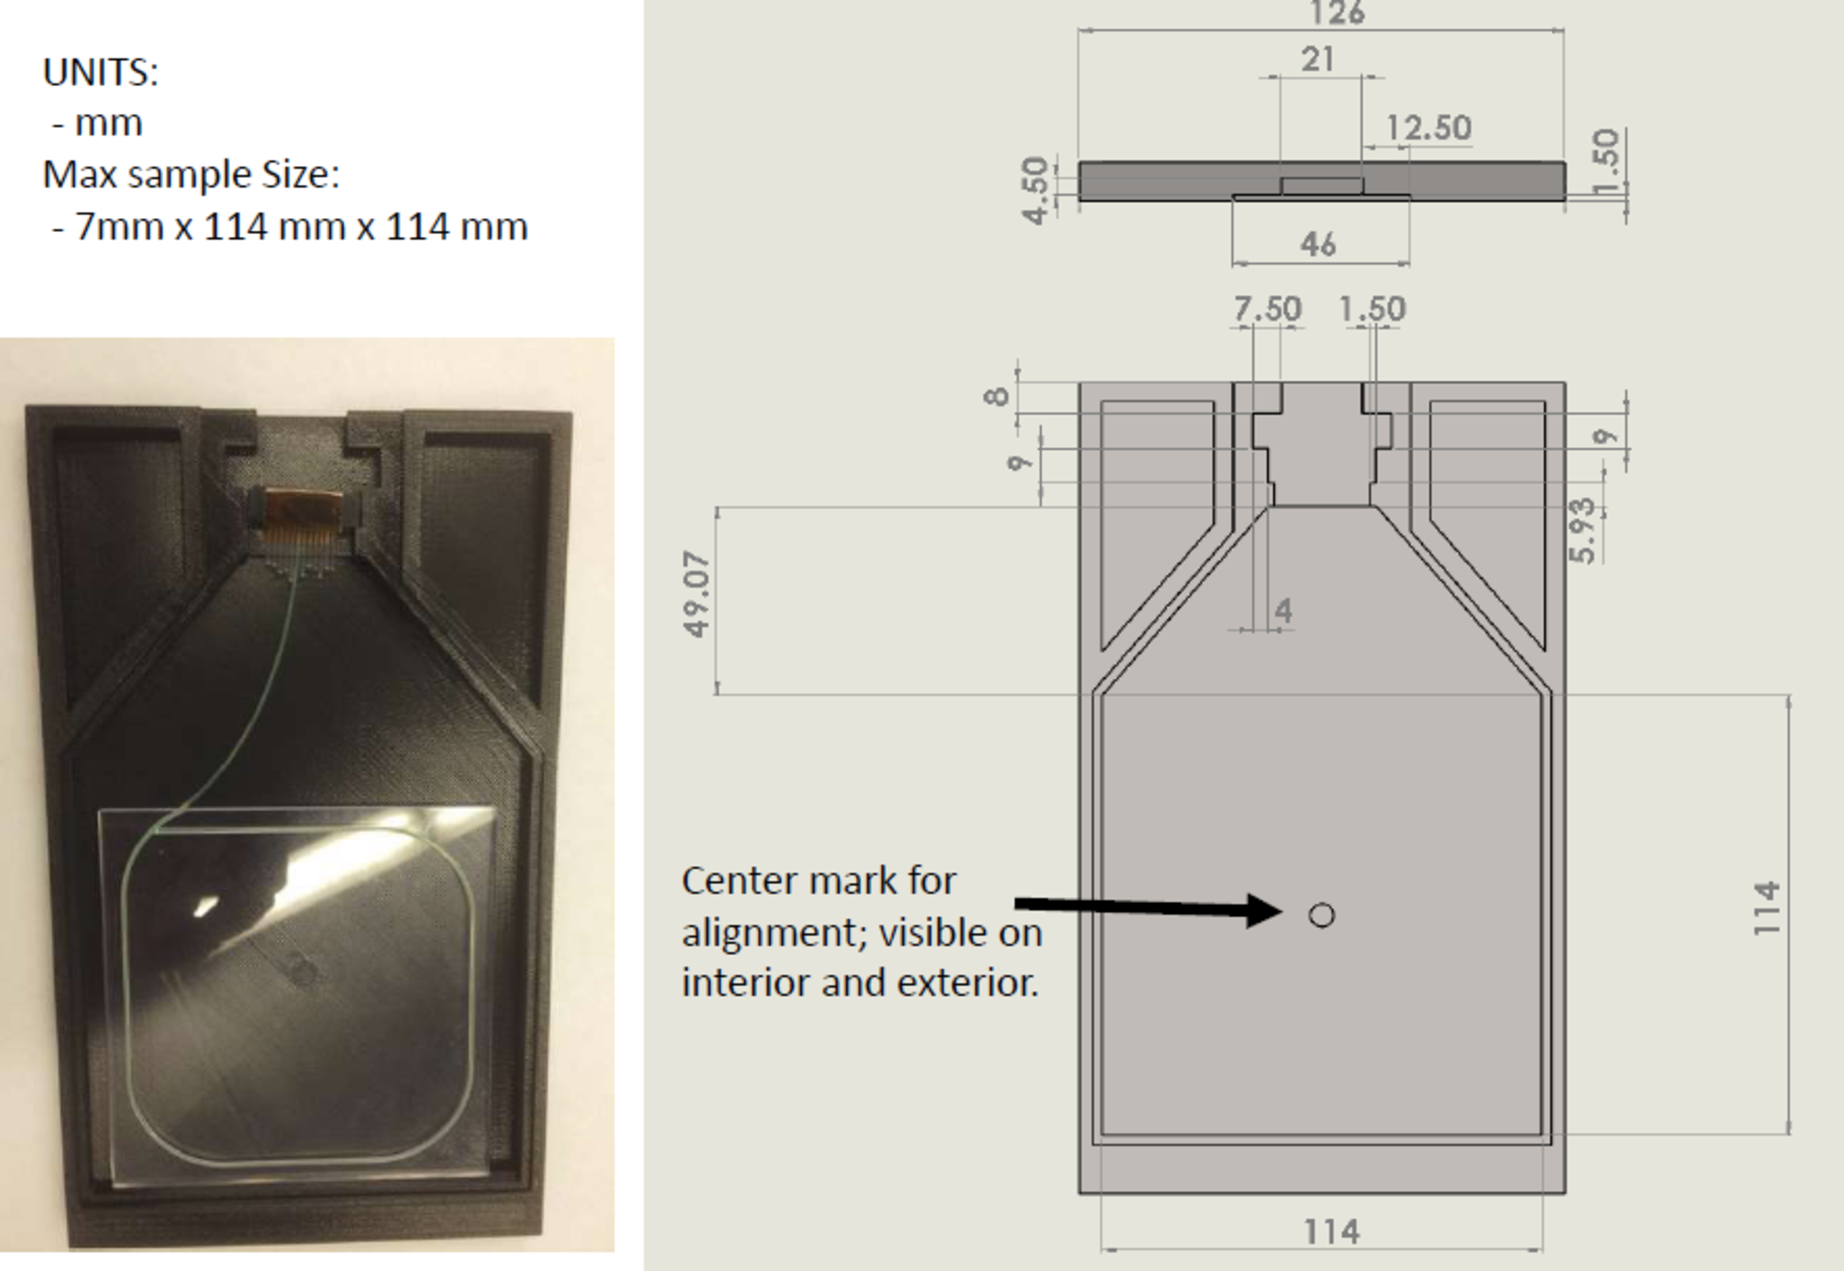
\includegraphics[width=0.5\textwidth]{./figures/samplemount.pdf}
  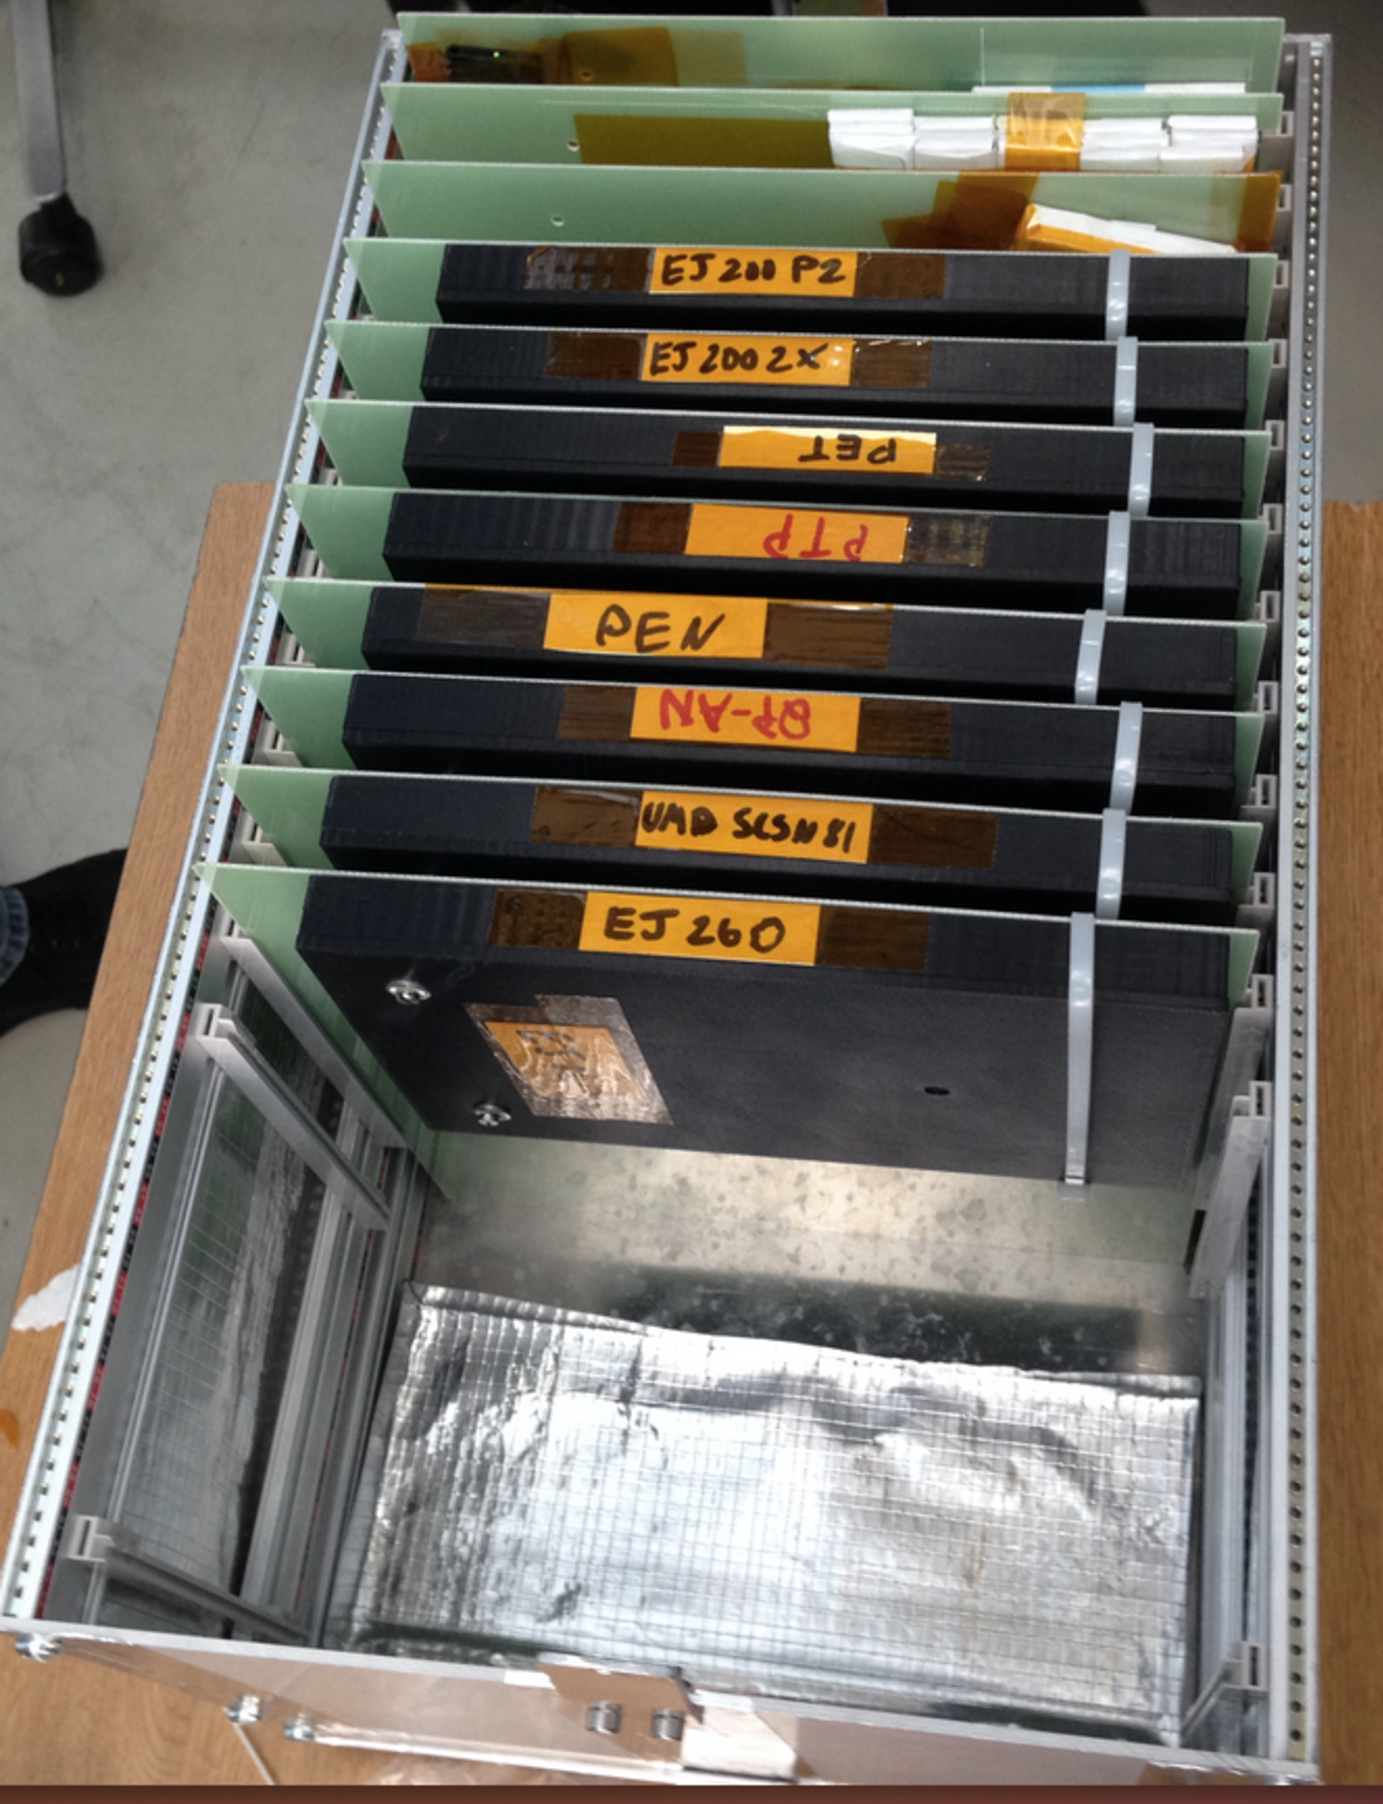
\includegraphics[width=0.5\textwidth]{./figures/hanging.pdf}
\caption{Design for fiber glass holder used for irradiations/
}
\label{fig:tiledesign}
\end{center}
\end{figure}


The dose was measured using FWT-60-00 Radiochromic dosimeters (thin films) by Far West Technology, RADMON detectors produced by CERN PPD,  and using Silicon Diodes.  The FWT dosimeters are attached directly to the scintillator samples.


The samples were installed during June of 2015.  The samples were removed
and measurements were made on {\color{red} put dates here}.

\section{Tile designs}
\label{sec:design}

{\color{red} put description of tested tiles here}


\section{Measurement techniques}
\label{sec:techniques}

The light output before and after irradiation in the CMS collisions hall
was measured using two different ways.

In the primary method measures, the response
of the scintillator was measured 
using a columnated beta source {\color{red} which one?}.
A SiPM (Hamamatsu {\color{red} I don't know}) was used as the photodetector.
The scintillator was places in a dark box, and a clear fiber was used
to connect it to the photodetector, outside the box.
The resulting current was measured using a Keithley 2001 or 6487 picoameter.
The SiPM was calibrated by plotting the dark current versus bias voltage and locating the break down voltage.  The data was taken with a bias voltage one volt above the breakdown.   The temperature was also monitored.

A secondary measurement measured the
light output produced by cosmic rays.
Scintillator-based counters above and below the tile were used for triggering.
  No attempt was made to select minimum ionizing (mip) muons.  The muons were thus
of low energy and produce more light than mips.

\section{Results}
\label{sec:Results}


\section{Conclusions}
\label{sec:Conclusions}

We presented results on radiation damage to scintillating materials
in 


\section{Acknowledgments}
The authors would like to thank Randy Ruchti of Notre Dame for
providing the capillaries.
 We would like to thank the University of Maryland
FabLab, especially {\color{red} who helped}, for help with fiber sputtering.
This work was supported in part by U.S. Department of Energy
Grant DESC0010072.

\section*{References}

\bibliography{acastorbox}

\end{document}
